\setstretch{1.4}
\sectiontitle{5}{Tip Tracking Integration}
\lhead{Tip Tracking Integration} % section header
An algorithm for capturing and processing the images from the cameras was previously developed by another student. This code was written in python and aims to deduce the position and direction of the tip of the ribbon while it moves in the brain phantom effectively "Tip Tracking". However, this code had not been developed for real-time use, but rather post-processing of videos.  Therefore it had to be refactored and somewhat rewritten for this project. Since the tip data acquired by this algorithm is necessary for the closed-loop path following control system, a method of sharing this data in real time with the C++ control system developed in Qt also had to be developed. This section therefore details the refactoring and communication implementation necessary to allow for live vision-feedback.



\lhead{Tip Tracking Integration - Methods} % section header
\subsection{Methods}

\subsubsection{Vision Code Refactoring Methodology}
The existing Python-based 3D tip tracking algorithm was implemented in a single file and had not been developed for real-time use. The system also needed additional functionality such as image capturing and communication to the Qt-based control system. Therefore it was decided that the code had to be restructured and altered. This was done according to the same code quality criteria discussed in the theory section in the Software Refactoring chapter. Additionally to make it suitable for real-time feedback the system was threaded. This was necessary due to the original system's reliance on YOLO \cite{redmon_you_2016}, a deep learning-based object detection algorithm, which is too computationally heavy for non-threaded real-time use.

\subsubsection{Switching to 2D Tip Tracking}
As the project progressed it became clear that even after refactoring the 3D vision system did not perform well enough for real-time vision. This was due to the computationally heavy step of running each frame through YOLO, limiting the system significantly, even after assigning it to its own thread. There were also other issues, such as the system having been trained previously on images of the ribbon moving in agarose instead of the bovine gelatin used for this thesis.As can be seen in figure \ref{fig:side_by_side} the images in the different mediums differ significantly. This resulted in poor detection and to jumps in estimation of the tip position and direction.
\begin{figure}[htbp]
    \centering
    \begin{subcaptionbox}{Picture of ribbon in agarose annotated with tip and pre-tip detections\label{fig:left}}[0.45\linewidth]
        {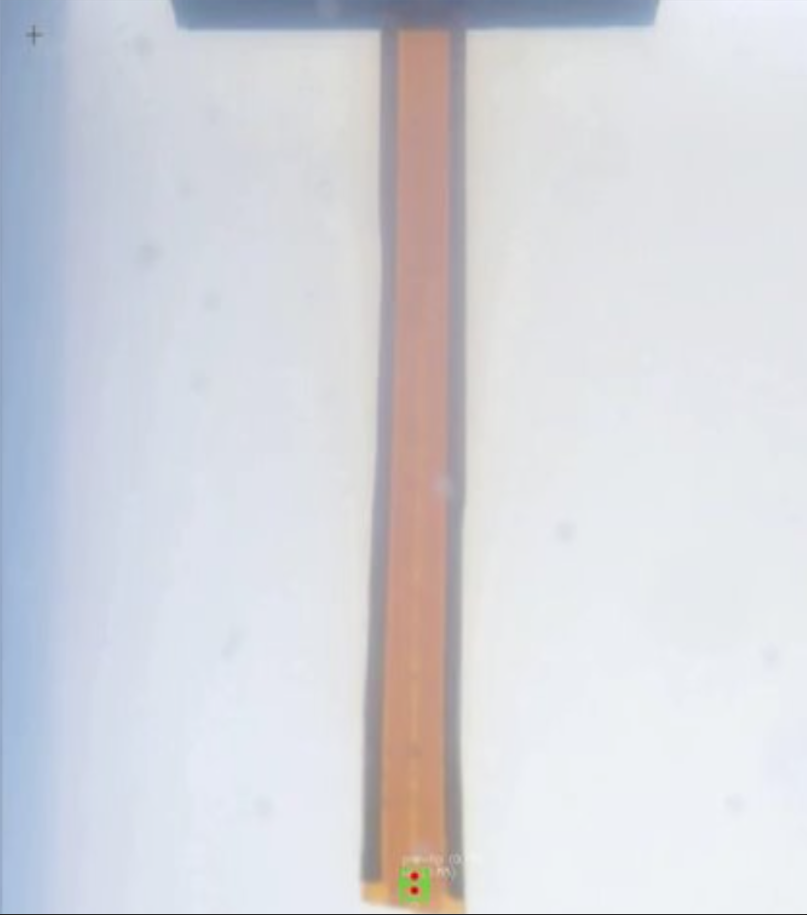
\includegraphics[width=\linewidth]{images/RibbonPicture/agarose2.PNG}}
    \end{subcaptionbox}
    \hspace{0.05\linewidth}
    \begin{subcaptionbox}{Picture of ribbon in bovine gelatin\label{fig:right}}[0.45\linewidth]
        {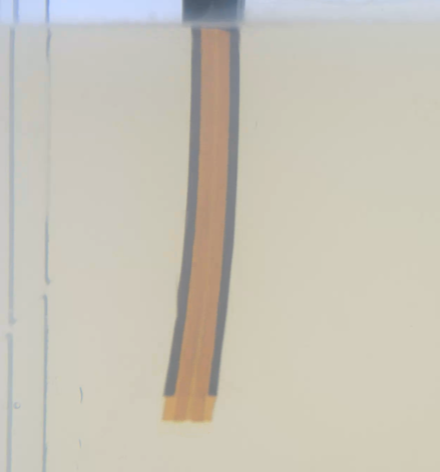
\includegraphics[width=\linewidth]{images/RibbonPicture/gelatin2.PNG}}
    \end{subcaptionbox}
    \caption{Pictures of the ribbon being inserted into an agarose brain phantom (a) vs a bovine gelatin brain phantom (b)}
    \label{fig:side_by_side}
\end{figure}
However 3D vision was not necessary for this thesis, therefore Lorenzo Noseda developed a 2D version that instead utilizes classical thresholding and skeletonization of the images. A new version of the refactored real-time 3D tip tracking was thereafter developed for this thesis, where the 2D tip detection was inserted into the structure instead of the 3D YOLO detection.

\subsubsection{Choosing a Communication Protocol}
In order to establish a robust connection between the already existing Python-based tip tracking system and the C++/Qt-based control system several ways of establishing an interface were evaluated (for a theory section on the relevant communication protocols see the appendix). In order to choose the most suited communication method a set of evaluation criteria based on their suitability for real-time data streaming \textit{Designing Data Intensive Applications} \cite{kleppmann_designing_2017} were used.

\begin{enumerate}
    \item \textbf{Latency and Real-Time Performance} - The ability to provide low-latency communication suitable for real-time control.
    \item \textbf{Fault Tolerance and Robustness} - Resilience to failures such as dropped messages or system crashes.
    \item \textbf{Communication Model} - Suitability for push-based (streaming) or pull-based (request-response) communication
    \item \textbf{Ordering and Consitency Guarantees} - The ability to ensure data arrives in the correct order.
    \item \textbf{Scalability} - The capability to accommodate future system expansions, such as integrating communication with a potential real-time path planning algorithm.
    \item \textbf{Ease of Implementation and Maintenance} - Complexity of integrating the communication method into the existing system.
\end{enumerate}

\lhead{Tip Tracking Integration - Design} % section header
\subsection{Design}
\subsubsection{Final Choice of Communication Protocol}
The methods discussed in the theory section in the appendix were all considered for enabling communication. File-based communication was ruled out early due to high latency and non-robust performance. Shared memory and named pipes offer better performance but had limited scalability and poor cross-platform/language compatibility. Message queues were also excluded as their high reliability and fault tolerance came at the cost of increased latency.

ZeroMQ was selected because it offers a lightweight, high-performance messaging layer with built in support for communication patterns such as publish/subscribe and request/reply \cite{lauener_how_2018}. The pub/sub pattern is especially useful here, as it allows the vision system to broadcast real-time data to the control system. This may also be easily expanded later one so that for example a real-time path planning algorithm can simply subscribe to the vision data.

To further reduce latency, ZeroMQ was configured to use UDP instead of TCP in order to avoid delays caused by retransmission. This makes it suitable for real-time feedback where receiving the most recent data is the priority. 

\lhead{Tip Tracking Integration - Results} % section header
\subsection{Results}
\subsubsection{Final Refactored Vision System}

The final refactored system consists of five primary modules as shown in figure \ref{fig:visioncode}, each with clearly defined responsibilities. A description of each class and a sequence diagram that illustrates the real-time processing flow can also be found in the appendix.

The vision system captures synchronized video streams from the Basler cameras at 10FPS. The detection pipeline developed by Lorenzo employs reference frame computation, morphological operations for noise reduction and iterative thinning algorithms to extract the centerline. This allows it to detect the tip position and reference point approximately 1mm proximal to the tip. A normalized direction vector is then computed based on these points. The coordinates, along with a normalized vector are formatted into a structure message which is then processed and sent by the communication class. In terms of threading the \texttt{ObjectDetector} and \texttt{CameraSystem} classes have dedicated worker threads with queue-based frame management. 

\begin{figure} [H]
    \centering
    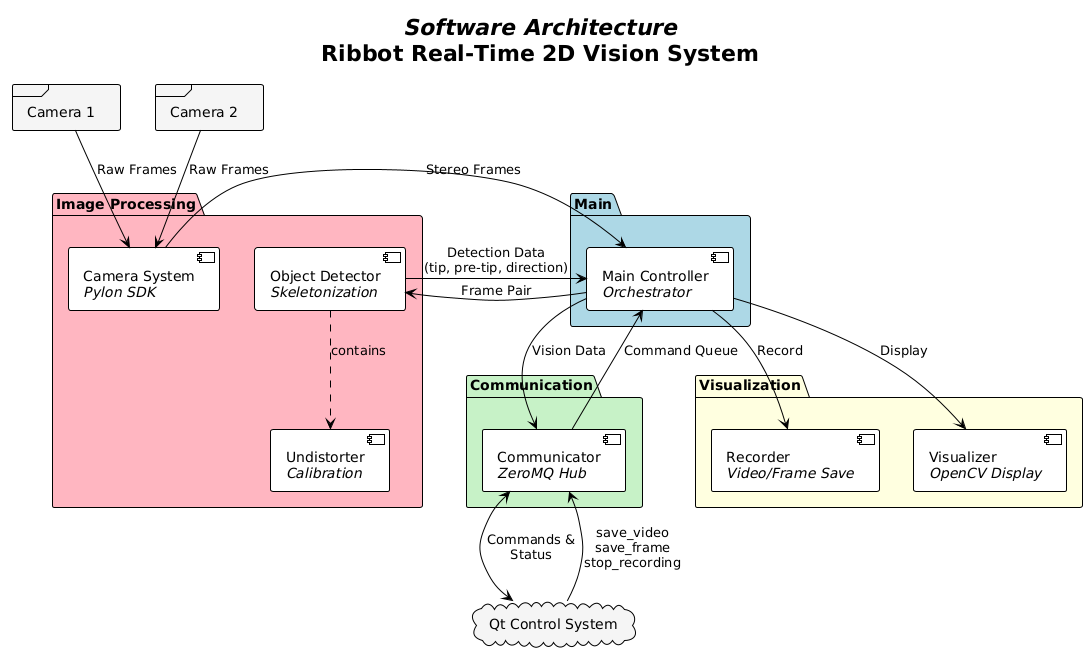
\includegraphics[width=\linewidth]{images/Software documentation/visionmodules.png}
    \caption{Modular architecture of the refactored vision system}
    \label{fig:visioncode}
\end{figure}

\subsubsection{Communication protocol between Python and Qt}
In the final communication system the Python based vision system acts as a publisher and continuously streams messages containing the timestamp, the two-dimensional coordinates of the detected tip and a point 1mm proximal to the tip, as well as a normalized direction vector. 

Before transmission, the coordinates are transformed from the vision system's coordinate frame to that used by the control system. The Qt based control system includes a dedicated subscriber thread that listens for updates on the specified ZeroMQ address. Once a message is received, the thread extracts the relevant information and updates the path following system with the latest tip and direction data. 

In addition to receiving data, the control system can also send commands to the vision module using a separate ZeroMQ DEALER socket. Three commands are currently implemented: \texttt{save\_video}, which starts recording video frames with an optional session tag; \texttt{stop\_recording}, which terminates the ongoing recording session; and \texttt{save\_frame}, which captures and stores a single image frame annotated with metadata. These commands allow the control system to trigger frame captures and recordings in sync with control events and to annotate them with relevant metadata. This enables accurate offline analysis and alignment of visual and control data logs.

\subsection{Discussion}
\subsubsection{Scalability}
The final implementation of the Vision system and its communication protocol to Qt is both scalable and flexible. Thanks to the publish/subscribe architecture, additional independent systems such as a possible future real-time path planner can simply subscribe to the vision data stream in the same way Qt does.

\subsubsection{Jumpy Detections}
While the current 2D vision system is functional for real-time feedback, the detections it produces are often visibly jumpy from frame to frame. This temporal inconsistency poses significant issues for closed loop control of the angle of the tip. This noise was therefore reduced by aggressive smoothing to avoid erratic control responses. 

Although this is a significant issue in the pathfollowing implementation it may not be worth extensive optimization for this iteration of the system. In future systems using fluoroscopy, the tip will likely be marked, potentially with a radiopaque marker, which would improve its visibility and result in more stable and consistent detections over time.

\subsubsection{Future extension to 3D Tip Tracking}
Although the current implementation uses a 2D vision pipeline, the system is fully prepared for expansion to 3D. The code is modularized such that this should be a straight forward process. As long as the output message contains the necessary position in the expected format, the communication to Qt would not have to be changed significantly either.

\subsection{Conclusion}
The refactored vision system and communication framework provide the necessary tip detection for real-time path following. It is modular, low-latency, and easily extendable for future developments, including 3D vision, improved tracking methods and additional data subscribers.

